\documentclass[twoside]{article}

%
% This is a borrowed LaTeX template file for lecture notes for CS267,
% Applications of Parallel Computing, UCBerkeley EECS Department.
% Now being used for CMU's 10725 Fall 2012 Optimization course
% taught by Geoff Gordon and Ryan Tibshirani.  When preparing 
% LaTeX notes for this class, please use this template.
%
% To familiarize yourself with this template, the body contains
% some examples of its use.  Look them over.  Then you can
% run LaTeX on this file.  After you have LaTeXed this file then
% you can look over the result either by printing it out with
% dvips or using xdvi. "pdflatex template.tex" should also work.
%

\setlength{\oddsidemargin}{0.25 in}
\setlength{\evensidemargin}{-0.25 in}
\setlength{\topmargin}{-0.6 in}
\setlength{\textwidth}{6.5 in}
\setlength{\textheight}{8.5 in}
\setlength{\headsep}{0.75 in}
\setlength{\parindent}{0 in}
\setlength{\parskip}{0.1 in}

%
% ADD PACKAGES here:
%

\usepackage{amsmath,amsfonts,graphicx}

%
% The following commands set up the lecnum (lecture number)
% counter and make various numbering schemes work relative
% to the lecture number.
%
\newcounter{lecnum}
\renewcommand{\thepage}{\thelecnum-\arabic{page}}
\renewcommand{\thesection}{\thelecnum.\arabic{section}}
\renewcommand{\theequation}{\thelecnum.\arabic{equation}}
\renewcommand{\thefigure}{\thelecnum.\arabic{figure}}
\renewcommand{\thetable}{\thelecnum.\arabic{table}}

%
% The following macro is used to generate the header.
%
\newcommand{\lecture}[4]{
   \pagestyle{myheadings}
   \thispagestyle{plain}
   \newpage
   \setcounter{lecnum}{#1}
   \setcounter{page}{1}
   \noindent
   \begin{center}
   \framebox{
      \vbox{\vspace{2mm}
    \hbox to 6.28in { {\bf Econ 626: Quantitative Methods II
  \hfill Fall 2018} }
       \vspace{4mm}
       \hbox to 6.28in { {\Large \hfill Lecture #1: #2  \hfill} }
       \vspace{2mm}
       \hbox to 6.28in { {\it Lecturer: #3 \hfill Scribes: #4} }
      \vspace{2mm}}
   }
   \end{center}
   \markboth{Lecture #1: #2}{Lecture #1: #2}

   %{\bf Note}: {\it LaTeX template courtesy of UC Berkeley EECS dept.}

   {\bf Disclaimer}: {\it Zhikun is fully responsible for the errors and typos appeared in the notes.}
   \vspace*{4mm}
}
%
% Convention for citations is authors' initials followed by the year.
% For example, to cite a paper by Leighton and Maggs you would type
% \cite{LM89}, and to cite a paper by Strassen you would type \cite{S69}.
% (To avoid bibliography problems, for now we redefine the \cite command.)
% Also commands that create a suitable format for the reference list.
\renewcommand{\cite}[1]{[#1]}
\def\beginrefs{\begin{list}%
        {[\arabic{equation}]}{\usecounter{equation}
         \setlength{\leftmargin}{2.0truecm}\setlength{\labelsep}{0.4truecm}%
         \setlength{\labelwidth}{1.6truecm}}}
\def\endrefs{\end{list}}
\def\bibentry#1{\item[\hbox{[#1]}]}

%Use this command for a figure; it puts a figure in wherever you want it.
%usage: \fig{NUMBER}{SPACE-IN-INCHES}{CAPTION}
\newcommand{\fig}[3]{
      \vspace{#2}
      \begin{center}
      Figure \thelecnum.#1:~#3
      \end{center}
  }
% Use these for theorems, lemmas, proofs, etc.
\newtheorem{theorem}{Theorem}[lecnum]
\newtheorem{lemma}[theorem]{Lemma}
\newtheorem{proposition}[theorem]{Proposition}
\newtheorem{claim}[theorem]{Claim}
\newtheorem{corollary}[theorem]{Corollary}
\newtheorem{definition}[theorem]{Definition}
%\newtheorem{example}[theorem]{Example}
\newenvironment{proof}{{\bf Proof:}}{\hfill\rule{2mm}{2mm}}
\newenvironment{example}{{\bf Example:}}{\hfill\rule{2mm}{2mm}}

\newtheorem{remark}[theorem]{Remark}
%\newenvironment{remark}[1][Remark]{\begin{trivlist}\item[\hskip \labelsep {\bfseries #1}]}{\end{trivlist}}


% **** IF YOU WANT TO DEFINE ADDITIONAL MACROS FOR YOURSELF, PUT THEM HERE:

\newcommand\E{\mathbb{E}}
\newcommand\dd{\mathrm{d}}

\usepackage{hyperref}
\newcommand\pp{\partial}

\begin{document}
%FILL IN THE RIGHT INFO.
%\lecture{**LECTURE-NUMBER**}{**DATE**}{**LECTURER**}{**SCRIBE**}
\lecture{1}{August 27-29}{Prof. Daniel Levy}{Zhikun Lu}
%\footnotetext{These notes are partially based on those of Nigel Mansell.}
\footnotetext[1]{This note contains 3-days lectures. Visit \url{http://www.luzk.net/misc} for updates.}

\section{Some history} 

  \subsection{About the Bernoulli brothers} 

  \subsection{Brachistochrone problem} 
    Brachistochrone means \textit{shortest time}. Note that the shortest path is not the fastest one.

\section{Methods of solving dynamic optimization}
  \begin{enumerate}
    \item Calculus of variations (Newton, ...), 1696-1697
    \item Optimal control (Pontryign, ...), 1960-1961
    \item Dynamic programming (Bellman), 1957
  \end{enumerate}

\begin{example}
  Suupose that a firm receives an order for B units of a product to be delivered by time T. Its goal is to accomplish this at minimum cost.

  {\tt Assumptions}: Unit production cost rises linearly with the production rate, given by
  \[c_1 x'(t), c_1 > 0\]
  \begin{itemize}
    \item $x(t)$ - inventory accumulated by time t
    \item $x'(t)$ - production rate
    \item $c_2>0$ - unit cost of holding inventory per unit of time
  \end{itemize}

  Total cost:
  $$c_1 x'(t) x'(t) + c_2 x(t) = c_1 (x'(t))^2 + c_2 x(t)$$
  This is a continuous time problem:
  $$\min \int_0^T [c_1 (x'(t))^2 + c_2 x(t)] \mathrm{d}t$$
  $$\text{s.t.  } x(0) = 0, x(T) = B, x'(t) \geq 0 $$
\end{example}

{\bf Goal}: Find $x(t)$ which will minimize the total cost of production.

{\bf Guess}: One possible solution is to produce at a constant rate by setting $x'(t) = \frac{B}{T}$. This is indeed feasible:
\begin{equation}
  x(t) = \int_0^t \frac{B}{T} \mathrm{d}t = \frac{B}{T} t
\end{equation}
because $x(0) = 0$, $x(T) = B$, and $x'(t) \geq \frac{B}{T}$. In that case, 
\begin{equation}
  \int_0^T [c_1 (x'(t))^2 + c_2 x(t)] \mathrm{d}t = \int_0^T \left [c_1 (\frac{B}{T})^2 + c_2 \frac{B}{T}t \right ] \mathrm{d}t = \left [c_1 (\frac{B}{T})^2 t + c_2 \frac{B}{2T}t^2 \right ]{\Bigg |}_0^T = c_1\frac{ B^2}{T} + c_2 \frac{BT}{2}
\end{equation}

{\bf A Simplified Version}: Suppose that $c_2=0, c_1= 1$. The problem is still dynamic in nature. Now the problem becomes
$$\min \int_0^T (x'(t))^2 \mathrm{d}t$$
\begin{equation}
  \text{s.t.  } x(0) = 0, x(T) = B, x'(t) \geq 0
\end{equation}

\textbf{Discrete Approximation}: Let us convert (1.3) into discrete time setting. Divide the interval $[0, T] \in \mathbb{R}$ into $\frac{T}{k}$ segments with equal length of $k$.

\begin{center}
  \texttt{[Insert a graph here]}
\end{center}

\begin{itemize}
  \item Approximation of $x(t)$

  $x(t)$ can be approximated by polygonal line with verticies $y$ at the end point of each segment: 
  $$(0, 0), (k, y_1), (2k, y_2), ..., (T, B) $$.
  \begin{center}
  \texttt{[Insert a graph here]}
  \end{center}
  
  \item Approximation of $x'(t)$
  $$x'(t) \approx \dfrac{\Delta x}{\Delta t} = \dfrac{y_i - y_{i-1}}{k}.$$
\end{itemize}

Then the objective of the firm is to determine $y_i, i=1, ..., \frac{T}{k}-1$ (since the last period value $y_{\frac{T}{k}} = B$), which minimizes the following
$$\min \sum_{i=1}^{\frac{T}{k}} \left [ \frac{y_i - y_{i-1}}{k} \right ]^2 k$$
\begin{equation}
  y_0 = 0, y_{\frac{T}{k}} = B, y_i - y_{i-1} \geq 0
\end{equation}
(1.4) is the discrete analogue of (1.3).

\begin{itemize}
  \item FONC w.r.t. $y_i$:
  \begin{equation}
    2 \frac{y_i - y_{i-1}}{k} - 2\frac{y_{i+1} - y_{i}}{k} = 0 \iff y_i - y_{i-1} = y_{i+1} - y_{i} \text{ or } \Delta y_i = \Delta y_{i+1}
  \end{equation}
  \item The solution property:

  Each 'day' the firm produces the same amount $\longrightarrow$ optimal strategy is to produce at \texttt{the constant rate}. The analogue between (1.3) and (1.4) suggests that constant production rate might be optimal in the continuous case as well. 

  \begin{center}
    \texttt{[Insert a graph here]}
  \end{center}

\end{itemize}

\begin{claim}
  Constant production rate is optimal for the continuous time version, (1.3).
\end{claim}

\begin{remark}
  This should not be surprising since "$(1.3) = \lim\limits_{k\rightarrow 0} (1.4)$".
\end{remark}

\begin{proof}
  Let $z(t)$ be some other $C^1$ feasible path $\Longrightarrow$ $z(0) = 0$ and $ z(T) = B$.

  Define $h(t) \equiv z(t) - x(t)$. Here, $h(t)$ is called a deviation path, $z(t)$ is called a comparison path. Since both $x(t), z(t)$ are feasible, we have
  $$\begin{aligned}
    h(0) &= h(T) = 0 \\
    z(t) &= h(t) + x(t) \\ 
    z'(t)&= h'(t) + x'(t) = h'(t) + \frac{B}{T}
  \end{aligned}$$
  $$\begin{aligned}
    \int_0^T (z'(t))^2 \mathrm{d}t - \int_0^T (x'(t))^2 \mathrm{d}t &= \int_0^T \left (h'(t)+\frac{B}{T} \right )^2 \mathrm{d}t - \int_0^T \left ( \frac{B}{T} \right )^2 \mathrm{d}t\\
    &= \int_0^T \left [ (h'(t))^2 + 2 h'(t) \frac{B}{T} + (\frac{B}{T})^2 \right ] \mathrm{d}t - \int_0^T \left ( \frac{B}{T} \right )^2 \mathrm{d}t\\
    &= \int_0^T (h'(t))^2  \mathrm{d}t + \int_0^T 2 h'(t) \frac{B}{T} \mathrm{d}t\\
    &= \int_0^T (h'(t))^2  \mathrm{d}t + \left [2 h(t) \frac{B}{T}\right ] {\bigg |}_0^T\\
    &= \int_0^T (h'(t))^2  \mathrm{d}t + 2 \frac{B}{T} (h(T) - h(0) )\\
    &= \int_0^T (h'(t))^2 \geq 0
  \end{aligned}$$
\end{proof}

\section{Dynamic Optimization Framework}
In general, a path can be identified if we know 
\begin{enumerate}
  \item starting time ${\bf t_0}$
  \item starting state ${\bf x(t_0)}$
  \item direction of path ${\bf x'(t)}$
\end{enumerate}
In general, the simplest general calculus of variations problem:
$$\int_{t_0}^{t_1} F(t,x(t),x'(t)) \mathrm{d}t$$
\begin{equation}
  \text{s.t. } x(t_0) = x_0, x(t_1) = x_1
\end{equation}
\begin{itemize}
  \item x - choice vaiable, can be a vector
  \item we can have higher order derivatives
\end{itemize}

{\bf Note}: FONCs of a continuous (discrete) time dynamic optimization model is a differential (difference) equations of several orders.

\underline{August 28, 2018 \quad Continued}

{\bf Objective Function} 

Value of the variable of interest - utility or profits, addded up over time. Examples include
$$
\begin{aligned}
  \text{Discrete - } &\sum_{t=0}^\infty u(c_t), \sum_{t=0}^\infty \Pi(P_t)\\
  \text{Continuous - } &\int_{0}^\infty u(c(t)) \mathrm{d}t, \int_{0}^\infty \Pi(P(t)) \mathrm{d}t
\end{aligned}
$$

$$\sum_{t=0}^\infty u(c_t) = u(c_0)+u(c_1)+...$$

{\bf Discounting in Discrete Time}
\begin{itemize}
  \item $\beta =$ \texttt{discount rate}, $0< \beta <1$
  
  \item $\beta^t$ = \texttt{discount factor}
  
  \item {Life-time utility} = $\sum_{t=0}^\infty  \beta^t u(c_t)$\\
  Also called \texttt{Present Discountied Value of the lifetime utility (PDV)}
\end{itemize}

{\bf Discounting in Continuous Time}

If we invest \$P at interest rate r/year, then
\begin{itemize}
  \item after one year, $P + rP = (1+r)P$
  \item after two years, $(1+r)^2 P$
  \item after $t$ years, $(1+r)^t P$
\end{itemize}
If interest is paid twice a year, then
\begin{itemize}
  \item after 6 months, $P + \frac{r}{2}P = (1+\frac{r}{2})P$
  \item after 1 year,   $(1+\frac{r}{2})^2 P$
  \item after $t$ years, $(1+\frac{r}{2})^{2t} P$
\end{itemize}
Generally, if interest is paid m times per year, where the per period rate is $\frac{r}{m}$, then
\begin{itemize}
  \item after 1 year,   $(1+\frac{r}{m})^m P$
  \item after $t$ years, $(1+\frac{r}{m})^{mt} P$
\end{itemize}
In the limit, if we discount continuously, $m \longrightarrow \infty$:
\begin{equation}
  \lim_{m \rightarrow \infty} \left ( 1 + \frac{r}{m} \right )^{mt} = e^{rt}
\end{equation}
If we invest \$$P$ today at interest rate r, computed continuously, then the amount will grow to \$$Pe^{rt}$. Conversely, \texttt{today's value of time t} \$$P$ should be \$$Pe^{-rt}$. Hence, $e^{-rt} \equiv $ continuous time discount factor.
$$\Longrightarrow \max \int_{0}^\infty u(c(t)) e^{-\delta t} \mathrm{d}t, ~ t \in \mathbb{R}$$
\underline{Comments}
\begin{itemize}
  \item $0 < \delta < 1$ is the discount rate.
  \item $e^{- \delta t}$ is the discount factor.
  \item As $t \uparrow$, we have $e^{-\delta t} \downarrow$.
  \item Generally, $\delta = \delta(t)$. Uzawa (1961)
\end{itemize}

{\bf Depreciation} (Decay)

Say, the stock of capital depreciates at rate $b>0$
$$\Longrightarrow \frac{K'(t)}{K(t)} = -b$$
$$K'(t) + b K(t) = 0$$
\begin{center}
  First order linear differential equation
\end{center}
$$e^{bt}[K'(t)+bK(t)]=0$$
$$\int e^{bt}[K'(t)+bK(t)] \dd t  = C_1$$
$$e^{bt} K(t) +C_2 = C_1$$
$$K(t) = C_3 e^{-bt}$$
$\implies b$ is the exponential rate of depreciation. If $K(0) = C_3$ is known, then $K(t) = K(0)e^{-bt}$

{\bf Note}

If $K(100)$ is known, say $K(100) = C_3e^{-100b}$, then
$$K(t) = K(100)e^{(100-t)b}$$
\texttt{In discrete time}\\ 
$K_{t+1} = (1- \delta)K_t$, or $K_{t+1} - (1- \delta)K_t = 0$, which ia s first order linear difference equation.

\subsection{Dynamic Models} \begin{itemize}
  \item Infinite horizon v.s. finite horizon
  \item Discrete time v.s. continuous time
  \item Deterministic v.s. Stochastic
  \item Linear v.s. nonlinear
\end{itemize}

\section{Dynamic Programming}

Consider the following dynamic discret-time, infinite horizon, deterministic model:
\begin{equation}
  \max \quad \sum_{t=0}^\infty \beta^t u(C_t), \quad 0 < \beta <1
\end{equation}
\begin{equation}
  \text{s.t.} \quad C_t + I_t = f(K_t) 
\end{equation}

\begin{itemize}
  \item $K_t$ - accumulated by the end of period t-1
  \item Capital evolution equation:
        \begin{equation}
          \begin{aligned}
          K_{t+1} =& I_t + (1- \delta) K_t\\
          =& K_t - \delta K_t + I_t
        \end{aligned}
        \end{equation}
  \item Assumption:
        \begin{enumerate}
          \item $\delta = 1$
          \item disposible equipment
        \end{enumerate}
        \begin{equation}
          I_t = K_{t+1} \qquad\text{ (think about saving)} 
        \end{equation}
\end{itemize}
Then (1.9) becomes
\begin{equation}
  C_t + K_{t+1} = f(K_t)
\end{equation}
(1.8) \& (1.9) $\implies$
\begin{equation}
  \max \quad \sum_{t=0}^\infty \beta^t u(C_t)
\end{equation}
\begin{equation}
  \text{s.t.} \quad C_t + K_{t+1} = f(K_t) 
\end{equation}

\texttt{Choice variable}: $\{C_t\}_{t=0}^{\infty}$, and $\{K_{t+1}\}_{t=0}^{\infty}$ with $K_0$ given.

This is a dynamic programming problem. It's solutions are called \texttt{policy functions} because the solutions will offer rules about how to choose the optimal values of choice variables as functions of the state variables.

In our case, a policy function will be a rule that will tell the decision maker how to choose optimally $C_t$ and $K_{t+1}$, give $K_t$.

\subsection{Finite Horizon Version}
Consider a finite-horizon version of (1.13)-(1.14):
\begin{equation}
  \max \quad \sum_{t=0}^T \beta^t u(C_t)
\end{equation}
\begin{equation}
  \text{s.t.} \quad C_t + K_{t+1} = f(K_t) 
\end{equation}
where we choose $\{C_t, K_{t+1}\}_{t=0}^{T}$.

Notice the recursive structure of the dynamic programming problem: Each period's decision problem is identical to other periods' decision problems, thus we can treat a given dynamic programming problem as a sequence of static problems.

\begin{center}
  \texttt{Bellman's insight}\\
  \texttt{[Insert a graph here]}
\end{center}

%{\bf A Lagrangian Approuch}: 
Plug (1.16) in to (1.15)
\begin{equation}
  \max_{\{K_{t}\}_{t=1}^{T}} \quad \sum_{t=0}^T \beta^t u( f(K_t) - K_{t+1})
\end{equation}

FONC w.r.t. $K_{t+1}$:
\begin{equation}
  - \beta^t u'(f(K_{t}) - K_{t+1}) + \beta^{t+1} u'(f(K_{t+1})-K_{t+2})f'(K_{t+1}) = 0
\end{equation}
which applies to $ t < T$, since $K_{T+1}$ is useless. Rewrite the FONC
\begin{equation}
   u'(f(K_{t}) - K_{t+1}) = \beta u'(f(K_{t+1})-K_{t+2})f'(K_{t+1})
\end{equation}
which is a \texttt{second-order difference equation}.

Using $C_t = f(K_{t}) - K_{t+1}$, we can get \texttt{the Euler equation}
\begin{equation}
  u'(C_t) = \beta u'(C_{t+1})f'(K_{t+1}).
\end{equation}

\begin{center}
  \texttt{Two Period Model}\\
  \texttt{[Insert a graph here]}
\end{center}

{\bf The Last Period}

When t = T, the last period, we will want to consume everything because there is no tormorrow.
\[
K_{T+1} = 0 \Longrightarrow C_{T+1} = f(K_T)
\]
Thus our problem becomes
\begin{equation}
  \max \quad \sum_{t=0}^T \beta^t u(C_t)
\end{equation}
\begin{equation}
\begin{aligned}
  \text{s.t.} \quad C_t + K_{t+1} = f(K_t) \\
  K_0 \text{~given and~} K_{T+1} = 0
\end{aligned}
\end{equation}

\begin{example}
  Let $u(C) = \ln C$, $f(K) = K^\alpha$, $0< \alpha <1$, then the Euler equation becomes  
  \begin{equation}
    \frac{1}{C_t} = \frac{\beta}{C_{t+1}}\alpha K_{t+1}^{\alpha-1}
  \end{equation}
  \begin{equation}
    \text{or \qquad} \frac{1}{K_{t}^\alpha - K_{t+1}} = \frac{\beta}{K_{t+1}^\alpha - K_{t+2}}\alpha K_{t+1}^{\alpha-1},
  \end{equation}
  which is (1.19) with specific utility and production functions.
  \begin{equation}
  \begin{aligned}
    & \frac{1}{ K_{t}^\alpha - K_{t+1} } = \frac{\beta}{K_{t+1}^\alpha - K_{t+2}}\alpha K_{t+1}^{\alpha-1}\\
    \iff & \frac{ \frac{1}{K_{t}^\alpha} }{\frac{1}{K_{t}^\alpha}(K_{t}^\alpha - K_{t+1})} = \frac{\alpha \beta \frac{1}{K_{t+1}^\alpha} K_{t+1}^{\alpha-1} }{\frac{1}{K_{t+1}^\alpha}(K_{t+1}^\alpha - K_{t+2})} \\
    \iff & \frac{ 1 }{{K_{t}^\alpha}} \frac{1}{1- \frac{K_{t+1}}{K_t^\alpha} } = \frac{\beta}{1- \frac{K_{t+2}}{K_{t+1}^\alpha}} \alpha \frac{K_{t+1}^{\alpha-1}}{K_{t+1}^\alpha}
  \end{aligned}
  \end{equation}
  Define $w_t \equiv \frac{K_{t+1}}{K_t^\alpha} = $ saving rate, then
  \begin{equation}
    \Longrightarrow \frac{w_t}{1- w_t } = \frac{\alpha \beta}{1- w_{t+1}}  
  \end{equation}
  We have transformed the original 2nd order difference equation into a 1st order difference equation system
  \begin{equation}
  \begin{cases}
    \dfrac{w_t}{1- w_t } = \dfrac{\alpha \beta}{1- w_{t+1}} \\
    w_t = \dfrac{K_{t+1}}{K_t^\alpha}
  \end{cases}
  \end{equation}

(1.26) can be rewritten as 
\begin{equation}
  w_{t+1} = 1 + \alpha \beta - \alpha \beta \frac{1}{w_t}
\end{equation}
Plot it with $\alpha = 0.8, \beta = 0.8$:
\begin{equation}
  w_{t+1} = 1.6 - \frac{0.64}{w_t}
\end{equation}

\begin{figure}[htbp] 
    \centering
    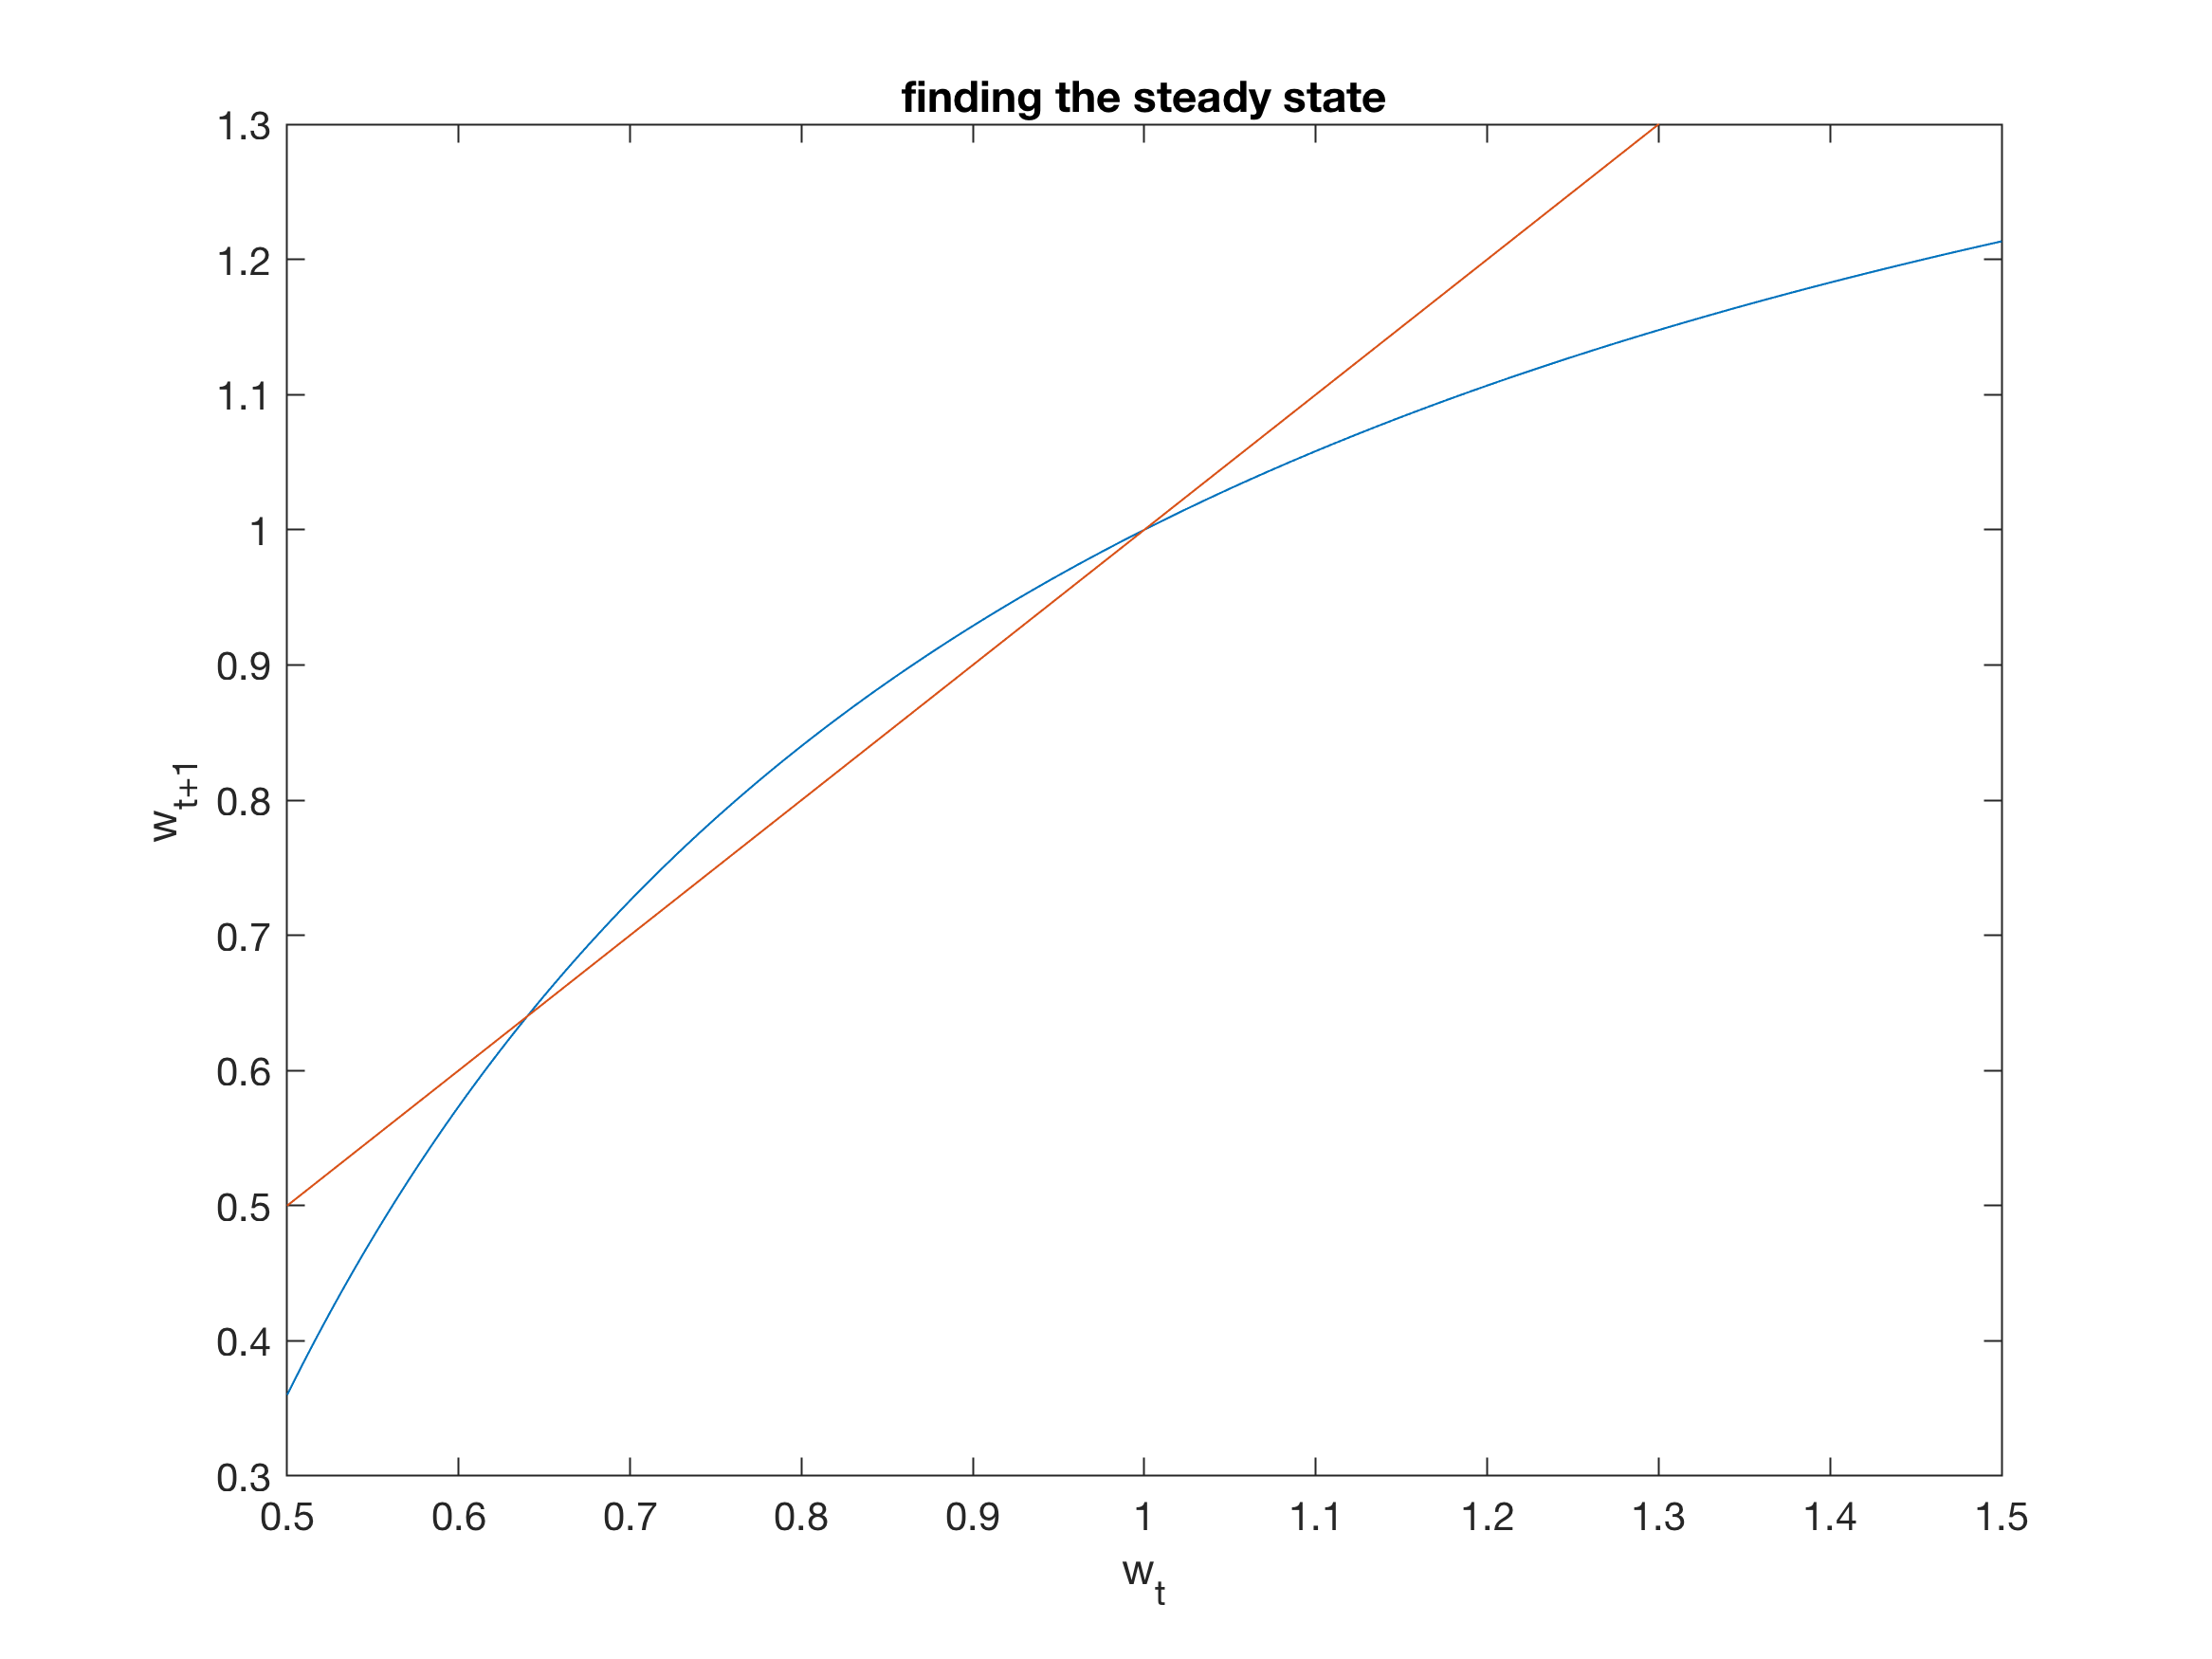
\includegraphics[width=.5\textwidth]{figure/wt.png}
    %\includegraphics[width=2in]{XeTeX-2.jpg} 
    \caption{The red line is the 45-degree line and the two intersections are possible steady states.}
\end{figure}

Let $w_{t+1} = w_t = w^*$, solving $w = 1+ \alpha \beta -  \frac{\alpha \beta}{w}$ yields
\begin{equation}
  w_{1,2} = \begin{cases}
    \dfrac{(1+ \alpha \beta) + \sqrt{(1+ \alpha \beta)^2-4 \alpha \beta}}{2} = 1 \\
    \dfrac{(1+ \alpha \beta) - \sqrt{(1+ \alpha \beta)^2-4 \alpha \beta}}{2} = \alpha \beta
  \end{cases}
  \end{equation}
However, $w$ cannot be 1. It is not optimal because it means that consumption equals zero, which does not make sense. We rule it out. Hence, 
\begin{equation}
  w^* = \alpha \beta
\end{equation}
To proceed, let us compute $w$'s a follows:
\begin{equation}
  w_t = \frac{K_{t+1}}{K_t} \Longrightarrow \frac{K_{T+1}}{K_T} = 0
\end{equation}
since $K_{T+1} = 0$.

As we are working backwards, rewrite (1.26) as 
\begin{equation}
  w_{t} = \frac{\alpha\beta}{1+\alpha\beta-{w_{t+1}}}.
\end{equation}
Hence
\begin{eqnarray}
  w_{T-1} &=& \frac{\alpha\beta}{1+\alpha\beta- w_{T}} =  \frac{\alpha\beta}{1+\alpha\beta}\\
  w_{T-2} &=& \frac{\alpha\beta}{1+\alpha\beta- w_{T-1}} = \frac{\alpha\beta}{1+\alpha\beta- \frac{\alpha\beta}{1+\alpha\beta}} = \frac{\alpha\beta + (\alpha\beta)^2}{1+\alpha\beta + (\alpha\beta)^2}\\
  w_{T-3} &=& \frac{\alpha\beta}{1+\alpha\beta- w_{T-2}} 
  =  \frac{\alpha\beta}{1+\alpha\beta - \frac{\alpha\beta + (\alpha\beta)^2}{1+\alpha\beta + (\alpha\beta)^2}}  
  = \frac{\alpha\beta + (\alpha\beta)^2 + (\alpha\beta)^3 }{1+\alpha\beta + (\alpha\beta)^2 + (\alpha\beta)^3}\\
  &\text{(by}& \text{guess and verify)} \notag\\
  w_{T-4} &=& \frac{\alpha\beta}{1+\alpha\beta- w_{T-3}} 
  = \frac{\alpha\beta + (\alpha\beta)^2 + (\alpha\beta)^3 + (\alpha\beta)^4 }{1+\alpha\beta + (\alpha\beta)^2 + (\alpha\beta)^3 + (\alpha\beta)^4}\\
  &\vdots& \notag\\
  w_{T-t} &=& \frac{\sum_{s=0}^{t} (\alpha\beta)^s - 1}{\sum_{s=0}^{t} (\alpha\beta)^s} \qquad (t = 1,2,\dots, T-1)\\
  &\vdots& \notag\\
  w_1 &=& w_{T-(T-1)} = \frac{\sum_{s=0}^{T-1} (\alpha\beta)^s - 1}{\sum_{s=0}^{T-1} (\alpha\beta)^s}\\
  w_0 &=& w_{T-T} = \frac{\sum_{s=0}^{T} (\alpha\beta)^s - 1}{\sum_{s=0}^{T} (\alpha\beta)^s}
\end{eqnarray}
By re-labelling, we can get the general formula for $0 \leq t \leq T-1$:
\begin{equation}
  w_{t} = \frac{\sum_{s=0}^{T-t} (\alpha\beta)^s - 1}{\sum_{s=0}^{T-t} (\alpha\beta)^s}
\end{equation}
Recall $\sum\limits_{s=0}^{n} b^s = \dfrac{1-b^{n+1}}{1-b}$, and we can rewrite (1.41):
\begin{equation}
  w_{t} = \frac{\sum_{s=0}^{T-t} (\alpha\beta)^s - 1}{\sum_{s=0}^{T-t} (\alpha\beta)^s} = w_{t} = \frac{\dfrac{1-(\alpha\beta)^{T-t+1}}{1-(\alpha\beta)} - 1}{\dfrac{1-(\alpha\beta)^{T-t+1}}{1-(\alpha\beta)}} = \frac{\alpha \beta - (\alpha\beta)^{T-t+1}}{1- (\alpha\beta)^{T-t+1}}, \quad t = 0, 1, \dots, T-1.
\end{equation}
Recall $w_t = \frac{K_{t+1}}{K_t^\alpha}$, we have
\begin{equation}
  K_{T+1} = {w_T}{K_t^\alpha} =  \frac{\alpha \beta - (\alpha\beta)^{T-T+1}}{1- (\alpha\beta)^{T-T+1}} K_t^{\alpha} = \frac{\alpha \beta - (\alpha\beta)^{1}}{1- (\alpha\beta)^{1}} K_t^{\alpha} = 0
\end{equation}
which is consistent with $K_{T+1} = 0$.

Now let $T \longrightarrow \infty$, $$\lim w_t = \alpha \beta = w^*$$

\end{example}

\subsection{Infinite Horizon Model}
Back to the infinite horizon model
\begin{equation}
  \max_{\{C_t, K_{t+1}\}_{t=0}^\infty} \quad \sum_{t=0}^\infty \beta^t u(C_t)
\end{equation}
\begin{equation}
\begin{aligned}
  \text{s.t.} \quad C_t + K_{t+1} &= f(K_t) \\
  K_0 & \text{~given}
\end{aligned}
\end{equation}

{\bf Note}: Since  this is an infinite horizon problem, we cannot proceed with backward recursion. 

Instead, we will use forward recursion. For this, we require \underline{additive-separability}:
\begin{equation}
  \sum_{t=s}^\infty u(C_t) = u(C_s) + \sum_{t=s+1}^\infty u(C_t) 
\end{equation}
which implies time-separability -- $MU(C_t) = MU(C_{t+1})$.

As we saw, 
\begin{equation}
  K_{t+1} = g(K_t), \quad t = 0, 1, \dots
\end{equation}
where $g : \mathbb{R}_+ \longrightarrow \mathbb{R}_+$ is the saving function, which is also called \texttt{policy function} in the language of Dynamic Programming.

\texttt{Value function} is the value of the objective function in optimum, i.e., the maximized value of the objective function.

By (1.47), we have 
\begin{eqnarray}
  K_1 &=& g(K_0)\\
  K_2 &=& g(K_1) = g(g(K_0)) \equiv \bar{g}(K_0)\\
  K_3 &=& g(K_2) = g(\bar{g}(K_0)) \equiv \bar{\bar{g}}(K_0)\\
  &\vdots& \notag
\end{eqnarray}

Hence the whole sequence of choice variables, ${\{C_t, K_{t+1}\}_{t=0}^\infty}$, depends on $K_0$, so does the the value function $V(\cdot)$:
\begin{equation}
  V(K_0) = \begin{cases}
  \max\limits_{\{C_t, K_{t+1}\}_{t=0}^\infty} \quad \sum_{t=0}^\infty \beta^t u(C_t)\\%, &\text{ if }case\\
  \qquad \text{s.t.} \quad C_t + K_{t+1} = f(K_t), \quad K_0  \text{~given}
  \end{cases}
\end{equation}

Let us simplify the problem by breaking it into two problems.

\begin{equation}
  V(K_0) = \begin{cases}
    \max\limits_{\{C_0, K_1\}} 
    \left [ u(C_0) + 
      \begin{cases}
        \max\limits_{\{C_t, K_{t+1}\}_{t=1}^\infty} \quad \sum_{t=1}^\infty \beta^t u(C_t)\\
        \qquad \text{s.t.} \quad C_t + K_{t+1} = f(K_t), \quad K_1  \text{~given}
      \end{cases}
    \right ] \\
    \qquad \text{s.t.} \quad C_0 + K_{1} = f(K_0), \quad K_0  \text{~given}
  \end{cases}
\end{equation}

Noticing that $ \begin{bmatrix}
        \max\limits_{\{C_t, K_{t+1}\}_{t=1}^\infty} & \sum_{t=1}^\infty \beta^t u(C_t)\\
        \text{s.t.} & C_t + K_{t+1} = f(K_t), \quad K_1  \text{~given}
      \end{bmatrix} = \beta V(K_1)$, we can write (1.52) as
\begin{equation}
  V(K_0) = \begin{cases}
    \max\limits_{\{C_0, K_1\}} 
    \Big \{ u(C_0) + 
      \beta V(K_1)
    \Big \} \\
    \qquad \text{s.t.} \quad C_0 + K_{1} = f(K_0), \quad K_0  \text{~given}
  \end{cases}
\end{equation}
or 
\begin{equation}
  V(K_0) = \max\limits_{\{K_1\}} \Big \{ u(f(K_0) - K_{1}) + \beta V(K_1) \Big \}
\end{equation}
which is \texttt{Bellman's equation}. BE is a functional equation, meaning the unknown is a function $V(\cdot)$.

{\bf Jargons}: In dynamic programming, as in optimal control:
\begin{enumerate}
  \item \texttt{State variable}: Ex. $K_0$
  \item \texttt{Control variable}: Ex. $K_1$
\end{enumerate}

\textbf{FONC} w.r.t $K_1$:
\begin{equation}
  - u'(f(K_0)-K_1) + \beta V'(K_1) = 0 
\end{equation}
\begin{equation}
  u'(f(K_0)-K_1) = \beta V'(K_1)
\end{equation}

\begin{theorem}[Envelope Theorem]
  Let $f(x,a)$ be the a $C^1$ function of $x \in \mathbb{R}^n$, where $a$ is some exogenously determined parameter, $a\in \mathbb{R}$, and consider the problem of maximizing the function $f(x,a)$. Suppose that $x^*(a)$ is an interior solution, where $x^*(a)$ is a $C^1$ function of $a$. Then
  \begin{equation}
  \begin{aligned}
    \frac{\dd }{\dd a}f(x^*(a),a) & = \sum_i \frac{\partial f}{\partial x_i}(x^*(a),a) ~ \frac{\dd x_i}{\dd a}(a) + \frac{\pp f}{\pp a}(x^*(a),a)\\
    & = \frac{\pp f}{\pp a}(x^*(a),a)
  \end{aligned}
  \end{equation}
\end{theorem}












%$$##
\clearpage
\section*{References}
%\beginrefs
%\bibentry{CW87}{\sc D.~Coppersmith} and {\sc S.~Winograd}, 
%``Matrix multiplication via arithmetic progressions,''
%{\it Proceedings of the 19th ACM Symposium on Theory of %Computing},
%1987, pp.~1--6.
%\endrefs

% **** THIS ENDS THE EXAMPLES. DON'T DELETE THE FOLLOWING LINE:

\end{document}





